% !Mode:: "TeX:UTF-8"
%!TEX program  = xelatex

%\documentclass{cumcmthesis}
\documentclass[withoutpreface,bwprint]{cumcmthesis} %去掉封面与编号页
\usepackage{url}
\title{论文标题}
\tihao{A}
\baominghao{4321}
\schoolname{东南大学}
\membera{卢立强}
\memberb{喻泽弘}
\memberc{杜昕昱}
\supervisor{老师}
\yearinput{2019}
\monthinput{05}
\dayinput{11}

\begin{document}

 \maketitle
 \begin{abstract}

这里是摘要

\keywords{\quad  聚类分析\quad   \quad  }
\end{abstract}

%目录
\tableofcontents

\section{问题提出与重述}

\subsection{问题的提出}

随着互联网的整体升级与手机行业的迅速发展,移动支付也逐渐得到普及,受到用户与商家的青睐。移动支付即通过手机而非现金或银行卡完成支付,具有移动性,及时性,定制化,集成性等特点,发展前景巨大,应用领域丰富。其中公交移动支付可以解决现金支付,刷卡支付等带来的不便,也可减少人工成本。

在出行领域相比于打车与共享单车,公交地铁的体量更大,交易量也十分可观,应用到移动支付行业会带来大量利润,所以通过分析市民乘车的支付行为建立盈利模型来分析与估计支付平台的商业盈利十分必要。



\subsection{问题的重述}

1.通过附件1,2给出的某市部分公交支付的信息与数据说明,分析该市乘车人的支付行为特征。

2.参考附件3的信息,建立第三方支付平台的商业盈利数学模型,定量分析第三方平台的收支和盈利情况。

3.通过附件1,2给出的该市四分之一的公交与地铁安装移动支付设备后试营运期间数据,估计该市实现全部公交移动支付后第三方平台的盈利情况。

\section{问题分析}

\subsection{问题的分析}

\textbf{问题一分析:}

为对用户的支付行为特征进行分析,我们分别用统计与聚类分析两个方法提取用户的支付行为特征并进行分析。分析附件一二给出的公交支付信息,发现其中有缺失数据与错误数据,需要先进行数据清洗与数据填充,得到有效数据。从而,我们需要先建立统计模型,通过建立哈希表对数据进行整理,分别从不同时间,不同个体等角度对用户的支付行为进行统计分析,得到统计数据,绘制出相应图表,根据图表与数据提取用户支付行为特征并尝试分析其原因。建立聚类分析模型,采用k-means方法对用户群体进行聚类,画出不同用户群体的月均出行次数与一天内各时间段的曲线图,分析图像得出不同用户的支付行为特征。

\textbf{问题二分析 :}

附件三给出了第三方支付平台的盈利模式,了解到第三方支付平台有手续费,广告费,沉淀资金的利息收入,服务费等多种盈利模式。其中每个盈利模式都有自己的方案,通过对每个盈利模式的方案进行分析,可以分别得到每种收益的表达式。支出方面分为机器成本,维护成本与推广费用几个方面,通过对第三方平台在各个环节产生的支出进行分析可得出每一项支出的表达式。平台盈利即为平台收入减平台支出。构建好平台盈利模型,通过定量分析的方法更改影响模型的因素,绘制盈利变化的曲线,分析收支与盈利情况。

\textbf{问题三分析 :}

公交移动支付覆盖率从该市四分之一扩展到全部,会对移动支付流量产生影响,进而影响第三方支付的盈利。针对客流量,可以通过一个城市的实例来找到不同线路客流量的比例。以南京市地铁为例,分析其中热门1/4线路与全部线路的客流量,得到热门1/4线路客流量占比,再通过模型一得到的有关移动支付份额数据,就可以对移动支付全覆盖之后该市移动支付的人数与交易额进行估算。将移动支付交易额带入第二问建立的模型中得到第三方平台盈利数据。根据模型一得出的支付行为特征,我们发现移动支付市场份额会随移动支付试运营的时间发生变化。通过模型一数据,可建立移动支付市场份额随时间增长的变化曲线,应用于模型二得出的盈利模型中,可建立移动支付覆盖率提升之后,平台盈利随时间变化的曲线,即可估计与分析该市在移动支付全覆盖后第三方支付平台的盈利情况。

\section{模型的假设}


\subsection{模型的假设}

\begin{itemize}
\item[(1)] 假设表中显示的支付时间均为有效时间,即乘客在支付时认为公交处于运营状态。
\item[(2)] 假设同一个人只能拥有一个ID。
\item[(3)] 假设移动支付试运营发生在该市客流量最大的$1/4$线路中。
\item[(4)] 假设南京地铁的部分运营数据可以反映该市公共交通的运营数据。
\item[(5)] 假设该市乘坐公交以及地铁的均价为2元。 
\item[(6)] 假设第三方支付平台资金周转能力良好。
\end{itemize}

\section{符号说明}
\begin{center}
\makeatletter\def\@captype{table}\makeatother
\begin{table}[h]
\centering
\caption{符号说明}\label{tab:aStrangeTable}\centering%添加标题 设置标签
\begin{tabular}{c|c|c}\hline
符号& 表示含义& 单位\\\hline
$SumCharge$ & 所有天数的公共交通支付笔数数目的总和 & \\
$SumCharge^{MobilePay}$ & 所有天数移动支付公共交通的成交量 & \\
%$MonthlyCharge_i$ & 第$i$月一周的公共交通支付数目的总和 &\\
%$MonthlyCharge^{MobilePay}_i$&第$i$月移动公共交通支付的笔数&\\
$DailyCharge_{(i,j)}$&第$i$月星期$j$的公共交通支付数目&\\
$DailyCharge^{MobilePay}_{(i,j)}$&第i月星期j当天移动支付公共交通的笔数&\\
%$\overline {times}$&人均乘车次数&\\
%$\overline {times_i}$&第$i$月人均乘车次数&\\
%$\overline {times}_{(i,j)}$&第$i$月星期$j$的人均乘车次数&\\
%$\overline {times}^{mobilePay}_{(i,j)}$&第$i$月星期$j$的人均移动支付公共交通笔数&\\
%$HourCharge_{i}$&一天第$i\sim i+1$小时内,公共交通的支付笔数&\\
%$HourCharge_{i}^{mobilePay}$&一天第$i\sim i+1$小时内,移动支付公共交通的笔数&\\
%$Uptime_{m}^{i}$&乘客$m$在时间段$i\sim i+1$的公交支付笔数, $0\leq i \leq 23$&\\
$CustomerSum(i)$&乘客$i$公共交通支付总量&\\
$CustomerSum(i)^{mobilePay}$&乘客$i$公共交通移动支付的数量&\\
$CustomerValidSum(i)$&乘客$i$有效公共交通支付总量&\\
$S_{sum}$&销售总额&RMB\\
$Pay_{sum}$&用户支付笔数&\\
$FreeRate$&第三方平台对用户的手续费率&\\
$ServiceRate$&第三方平台对商户的服务费率&\\
$adFree$&第三方平台向商户收取的广告费&RMB/CPM\\
$\overline {remain}$&用户人均余额&RMB\\
${NumberOfPeople}$&使用该第三方支付平台的人数&\\
$SedMoney(i)$&第i月的存入银行的沉淀资金&RMB\\
$SedMoney^j(i)$&第i月的沉淀资金经过$j$月以后的总额&RMB\\
$r=IncreaseRate$&沉淀资金的增长率&\\\hline
\end{tabular}
%\caption{这是一张三线表}\label{tab:aStrangeTable}  标题放在这里也是可以的
\end{table}
\end{center}



\section{模型建立与求解}
\subsection{问题一的建模与解答}
\subsubsection{数据清洗}
附件一,二给出了某市部分公交支付的信息与数据,分别取了2,5,8,11月份中连续的7天的支付信息,包括支付ID、上一次乘车交易时间、本次乘车时间、
付款方式,当月地铁与公交乘车次数与乘车总次数。每天大概有一百多万条乘车数据,而其中也有许多无效数据与错误数据,需要我们在统计前对数据进行清洗,现对数据进行以下三个方面的数据填充以及清洗:

1. 对于PAYTYPE值为Null的数据:将部分PAYTYPE项中的Null值替换为0。附件一中的PAYTYPE项表示的是支付方式,其中0代表公交移动支付,1代表公交卡支付,而通过附件2提供的信息可知Null为没刷卡,所以将Null将NULL算为非公交卡支付。通过观测2月、5月、8月和11月的公交数据可以发现,除二月以外的其他月中,
支付类型只为0,1和NULL,又因为NULL表示非公交卡支付,所以这里我们可以把NULL归为移动支付。对于二月的数据,我们可以把支付类型为NULL的数据,按比例分配给移动支付方式和其它支付方式。

2.对于UPTIME没有记录的数据:UPTIME中的0001-1-1表示没有刷卡记录,对这部分数据进行填充:

(1)若该乘客相同的月份的相邻两次记录中,前一次的UPTIME丢失,而后一次的乘车记录给出了LASTTIME,则我们使用后一次记录的LastTtime填充上一次记录的UPTIME。

(2)若找不到可以补充的LASTTIME,则按照以下步骤填充:

Step1:将乘客$i$所有有效乘车时间提取出来,构成数组$Uptime_i$[k](k=0,1...CustomerValidSum(i))。

Step2:在0$\sim$CustomerValidSum(i)范围内随机生成数字n。

Step3:将n当作数组下标在$Uptime_i$数组中取$Uptime_i$[n]作为填充数据。

Step4:对于多个Uptime缺失的,重复Step2$\sim$Step4步骤

3. 清理极少乘坐公交的人:对于$CustomerSum(i)\leq2$ 的乘客信息,由于他们乘坐公交次数很少,支付行为特征难以分析,或者不是该市市民,对于这种乘客的信息进行清理,删掉这条ID相关的信息。

\subsubsection{数据统计}

由于支付数据量很大,我们先遍历一边所有excel表格,根据每个人的ID构建哈希表储存他们的信息,根据有效数据整理出如下数据:

(1)每天的移动支付笔数:$\overline {times}^{mobilePay}_{(i,j)}​$

(2)每天的公交支付笔数:$\overline {times}_{(i,j)}$

(3)一天中每小时内公交支付笔数:$HourCharge_{i}$

(4)一天中每小时内公交移动支付笔数$HourCharge_{i}^{mobilePay}$

\subsubsection{支付行为模型}

1. 日均公交移动支付与总支付笔数小时分布图

统计平均一天中每小时内的公交支付总笔与移动支付的总笔数,绘制柱状图,其中移动支付笔数包含在总笔数之中。

2.公交移动支付与总支付笔数按日期分布图

统计每天的公交支付笔数与公交移动支付笔数,按日期增长顺序绘制折线图。

3.公交支付笔数星期内分布图

将四周的公交支付笔数分别按一星期七天画出四条折线图

4.移动支付占比随乘车次数分布图

计算乘车次数为i的乘客的移动支付笔数总和与总乘车次数和,之后求出乘车次数为i的移动支付笔数占总乘车次数比例,绘制移动支付占比随乘车次数增长的折线图。

5. 公交移动支付星期内分布图

将四周的公交移动支付笔数分别按一星期七天画出四条折线图

6.公交移动支付占比图

将四周每周的移动支付占比绘制饼图(4张)

\subsubsection{支付特征分析}

。。。
\subsubsection{聚类统计分析}
数据统计模型可以获得用户整体的支付行为特征,若想对用户群体进行分类,得到用户整体中具有各自支付行为特征的群体,就需要建立聚类分析模型,将用户群体进行划分。我们采用K-means 的聚类算法,对用户群体的支付行为特征进行聚类分析。

\textbf{K-means算法 :}K-Means算法是无监督的聚类算法,应用广泛。K-Means算法的思想为对于给定的样本集,按照样本之间的距离大小,将样本集划分为K个簇。让簇内的点尽量紧密的连在一起,而让簇间的距离尽量的大。应用于本题,我们要将用户整体划分为几个不同的群体,其中每个群体内部的支付行为特征相似,不同群体的支付行为特征不同。K-means算法流程如下:

Step1: 从数据集中随机选取K个样本作为初始聚类的中心$C={c_1,c_2,...,c_k}$

Step2: 针对数据集中每个样本$x_i$,计算它到K个聚类中心的距离并将其分到距离最小的聚类中心所对应的类中

Step3: 针对每个类别$c_i$,重新计算它的聚类中心$c_i=\frac{1}{\left|c_i\right|}\sum_{x \in c_i}x$(即属于该类的所有样本的质心)

Step4: 重复Step2和Step3直到聚类中心的位置不再变化

\textbf{K-means模型构建:}

本题应用于K-means模型中的特征,输入。。。

由构建的K-means算法得到核数为

图

\textbf{基于K-means的支付行为特征分析:}



\subsection{问题二的建模与解答}
\subsubsection{第三方支付平台的收入}
由附件三分析,第三方支付平台的收入主要由手续费,服务费,广告费,沉淀资金的利息几个部分组成。
\begin{figure}[h]
\centering
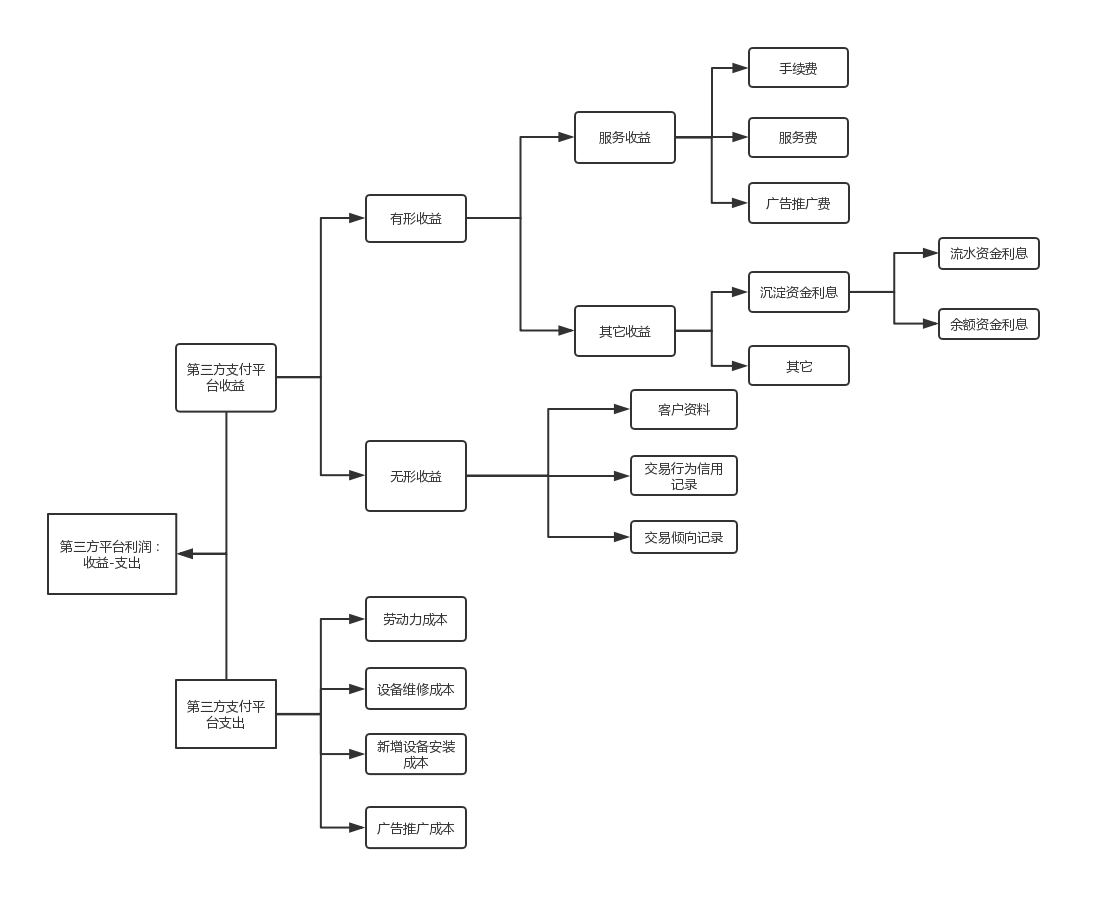
\includegraphics[scale=0.4]{profit.png}
\caption{盈利模型}
\end{figure}
现从以下四个方面构建收入模型:

1.手续费$T_1$:即第三方向用户收取手续费和向银行支付的手续费之差,无论是,线上支付的支付宝,还是线下支付的拉卡拉,手续费都是第三方支付平台的传统盈利方式。附件三中对手续费的区间描述为$0.08\%-1.25\%$,根据微信,支付宝等主流第三方支付平台的手续费率,在模型中取手续费率$FreeRate=0.1\%$。可得手续费$t_1$的表达式为:
\begin{equation}
T_1=S_{sum}*FreeRate
\end{equation}

2.服务费$T_2$:这里所指的服务费是指第三方支付平台为其客户提出支付解决方案,提供支付系统以及各种增值服务。这也应该是第三方支付平台最核的盈利模式。支付宝服务费为$0.6\%$,在模型中取服务费率$ServiceRate=​0.6\%$,可得服务费$T_2$表达式为:
\begin{equation}
T_2=S_{sum}*ServiceRate
\end{equation}

3.广告费$T_3$:为第三方平台向商户收取的广告费用。通过调查广告网站设定广告单价$adFree=40RMB/CPM$,单位为每一千人浏览广告的价格。广告费$T_3$的表达式为:
\begin{equation}
T_3=Pay_{sum}*adFree/1000
\end{equation}

4.沉淀资金$T_4$:沉淀资金即为备付金,为办理客户委托的支付业务而实际收到的预收货币代付资金。其中风险准备金比例不得低于其银行账户利息所得$10$%,这也就意味着第三方支寸机构最多可以获得$90$%的利息收入。在以活期存款形式的客户备付金满足日常支付业务的需要后,其他客户备付金可以“以活期存款、单位定期存款、单位通知存款、协定存款或经中国人民银行批准的其他形式"存放,但"期限不得超过3个月"。这意味着,部分客户备付金可转成为期3个月的单位定期存款。协议存款率为$4\%\sim5\%$,手续费估算为$0.78\%$,沉淀金包含长期沉淀金与短期沉淀金两个部分。长期沉淀金主要为用户在第三方平台的余额,而短期沉淀金为第三方平台的流水金额。

沉淀资金增长率的计算:设$r_1$为风险准备金比例,$a_1$为活期资金占总资金比例,$r_2$为三个月的活期年利率,$r_3$为协定年利率。沉淀资金的增长率
\begin{equation}
r=(1-r_1)(a_1*r_2+(1-a_1)*r_3)/12
\end{equation}

设$a_3$为发卡额的保有比例,$UserBalance(i)$表示经过$i$月以后,沉淀资金中用户余额总数的值,其中$UserBalance(0)$表示未放入银行获益前的用户余额总数。
\begin{equation}
UserBalance(0)=(\overline {remian} * {NumberOfPeople})*a_3
\end{equation}

第$i$月的流水资金用$SedMoney(i)$表示,$SedMoney^j(i)$表示第$i$月的流水资金经过$j$月以后的值,则$SedMoney^j(i)$的表达式为
\begin{equation}
SedMoney^j(i)=\left\{
\begin{aligned}
& (1+r)*(1-t_1)SedMoney^{j-1}(i) &j=3n-2&&j != 1\\
&(1+r)*SedMoney^{j-1}(i)  & j=3n-1or3n\\
&SedMoney(i)  & j=0\\
\end{aligned}
\right.
\end{equation}
\begin{equation}
UserBalance(i)=\left\{
\begin{aligned}
& (1+r)*(1-t_1)UserBalance(i-1) &j=3n-2&&j != 1\\
&(1+r)*UserBalance(i-1)  & j=3n-1or3n\\
\end{aligned}
\right.
\end{equation}
计算沉淀资金的年利润:
\begin{equation}
T_4=\sum_{i=0}^{12} SedMoney^{12-i}(i)-\sum_{i=0}^{12} SedMoney(i)+UserBalance(12)-UserBalance(0)
\end{equation}
其中,$\sum_{i=0}^{12} SedMoney^{12-i}(i)$表示年底时,每个月流水金额的值。$UserBalance(12)$表示年底时用户总余额的值。
\subsubsection{第三方支付平台的支出}
将平台的支出分为固定成本和推广成本

1. 固定成本$O_1$:主要体现为新增设备安装成本、维护设备成本以及劳动力成本三个部分。

设平均一台支付机器的价格为$V_{machine}$,机器数量为$N_{machine}$,机器维护均价为$V_{maintain}$员工工资支出为$S$,$C_1$的表达式为:
\begin{equation}
C_1=N_{machine}*(V_{machine}+V_{maintain})+S
\end{equation}

2. 推广费用$O_2$:主要体现为平台在各个媒体渠道投放广告用来提高平台的知名度以及市场份额

设投放广告数量为$N_{ad}$,广告均价为$V_{ad}$,$C_2$的表达式为:
\begin{equation}
C_2=N_{ad}*V_{ad}
\end{equation}

\subsubsection{第三方支付平台的盈利模型}
第三方平台的总盈利$W$:收入-支出
\begin{equation}
W=T_1+T_2+T_3+T_4-C_1-C_2
\end{equation}

结合表达式$1\sim10$可得:
\begin{equation}
\begin{split}
W=&S_{sum}*FreeRate+S_{sum}*ServiceRate+Pay_{sum}*adFree/1000\\&+\sum_{i=0}^{12} SedMoney^{12-i}(i)-\sum_{i=0}^{12} SedMoney(i)+UserBalance(12)-UserBalance(0)\\&-(N_{machine}*(V_{machine}+V_{maintain})+S)-N_{ad}*V_{ad}
\end{split}
\end{equation}

\subsubsection{问题二模型的求解}
\subsubsection{问题二模型的分析}
\subsection{问题三的建模与解答}
当该市的公交移动支付覆盖率从四分之一变为全部覆盖时,移动支付的人数会提高,通过附件一二的数据可以求出实施移动支付的公交地铁站的移动支付占比,但由于附件1与附件2 是该市四分之一的公交与地铁安装移动支付设备后试营运期间的数据,想要得到移动支付占比则需要知道1/4试运营站点中的移动支付的客流量占比$O_{1/4}$,现通过分析南京市地铁的客流量来计算$O_{1/4}$,其流程图如下:

\begin{figure}[h]
\centering
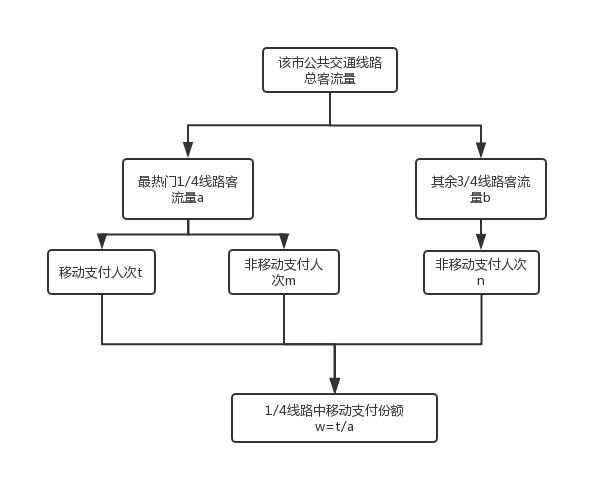
\includegraphics[scale=0.35]{flow.png}
\caption{移动支付占比计算}
\end{figure}
以南京市为例,我们通过查阅南京地铁集团跟踪评级报告获取到2017年度南京各地铁线路的客流量和里程数,我们假设移动支付试运营的1/4的线路取地铁线路客流量最大的1/4线路,由下表2给出了2017年南京各个线路的里程数与客流量的数据:
\begin{center}
\makeatletter\def\@captype{table}\makeatother
\begin{table}[h]
\centering
\caption{南京地铁线路}\label{tab:aStrangeTable}\centering%添加标题 设置标签
\begin{tabular}{c|c|c|c|c|c}\hline
线路&里程(km)&客流量(万人)&线路&里程(km)&客流量(万人)\\\hline
1号线&37.5&31241.59&10号线&21.2&4602.58\\
2号线&37.1&26288.11&S1号线&33.0&2267.29\\
3号线&43.9&24752.45&S3号线&35.5&117.33\\
4号线&32.6&4890.78&S8号线&44.4&3574.44\\\hline
\end{tabular}
\end{table}
\end{center}

根据表2中的数据绘制出各线路客流量比例和里程数比例。
\begin{figure}[h]
\centering
\begin{minipage}[c]{0.4\textwidth}
\centering
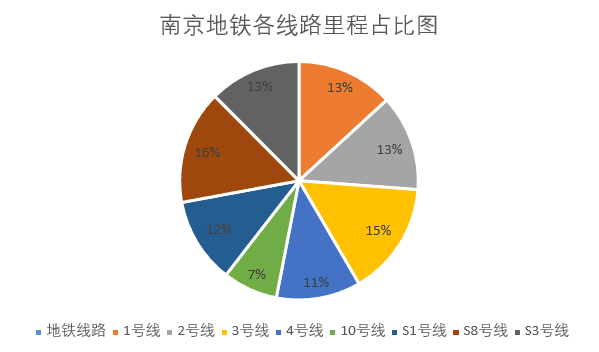
\includegraphics[height=4.5cm,width=7.5cm]{5.png}
\end{minipage}
\begin{minipage}[c]{0.4\textwidth}
\centering
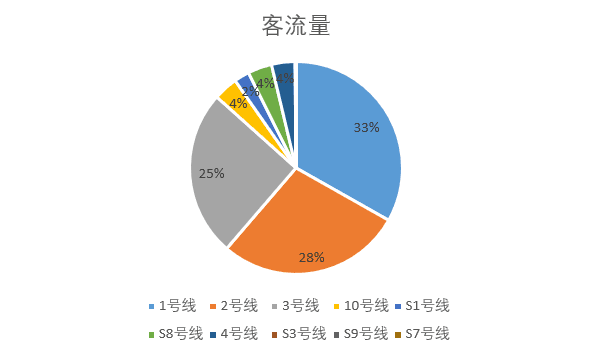
\includegraphics[height=4.5cm,width=7.5cm]{6.png}
\end{minipage}
\caption{南京地铁客流量占比}
\end{figure}

由图3我们可以发现一号线和二号线为客流量最多的两条铁路线路,且一二号地铁线的公里数总和占地铁总公里数的26\%,近似于1/4的铁路线路,符合模型中的场景,所以取一号线与二号线为试运营的1/4线路。设$P_i$为八条线路中第i条线路的客流量,$O_{1/4}$就等于计算一号线二号线的客流量占比即:
\begin{equation}
O_{1/4}=\frac{P_1+P_2}{\sum_{i=1}^{8}P_i}
\end{equation}

求出$O_{1/4}$后,将南京市的客流量占比应用到该市,可得到该市1/4试运营地点的客流量。设第i月第j天1/4线路中移动支付占比为$MobileProportion(i,j)$,则根据附件一,二的统计数据可得到$MobileProportion(i,j)$的表达式:

\begin{equation}
MobileProportion(i,j)=DailyCharge^{MobilePay}_{(i,j)}/(DailyCharge_{(i,j)}*O_{1/4})
\end{equation}

\subsubsection{问题三模型的建立}


\subsubsection{问题三模型的求解与分析}


\section{模型的评价}
\subsection{模型的优点}
\subsection{模型的缺点}
\subsection{模型的改进}
\section{模型的推广与应用}


%参考文献
\begin{thebibliography}{9}%宽度9
 \bibitem{bib:one} 王琛.第三方支付的主要盈利模式及存在的风险分析——以支付宝为例[J].商业文化,2015(18):166-168.
 \bibitem{bib:two}钱凯凯,蒋秀.从支付宝微信支付看第三方支付的盈利模式[J].商场现代化,2016(30):77-78.
 \bibitem{bib:three}孙吉贵,刘杰,赵连宇.聚类算法研究[J].软件学报,2008(01):48-61.
 \bibitem{bib:four}陈佳琪. 第三方支付平台的风险评估[D].湖南大学,2018.
 \bibitem{five}姚宁. 基于移动平台的第三方支付模式研究[D].华东理工大学,2016.
 \bibitem{bib:six}张念,王毅磊.中国移动支付发展的现状及问题——以支付宝为例[J].现代营销(下旬刊),2019(03):50.
 \bibitem{bib:seven}易涌征. 移动支付消费者接受的影响因素研究[D].浙江大学,2012.
 
\end{thebibliography}

\newpage
%附录
\begin{appendices}
\section{遗传算法--python 源程序}
\begin{lstlisting}[language=python]
print helloworld!
 \end{lstlisting}
 \section{程序--X代码}
\begin{lstlisting}[language=c]
cout<<"helloworld";
 \end{lstlisting}
\end{appendices}

\end{document} 